\documentclass[journal,12pt,twocolumn]{IEEEtran}
\usepackage{setspace}
\usepackage{gensymb}
\singlespacing
\usepackage[cmex10]{amsmath}
\usepackage{amsthm}
\usepackage{mathrsfs}
\usepackage{txfonts}
\usepackage{stfloats}
\usepackage{bm}
\usepackage{cite}
\usepackage{cases}
\usepackage{subfig}
\usepackage{longtable}
\usepackage{multirow}
\usepackage{enumitem}
\usepackage{mathtools}
\usepackage{steinmetz}
\usepackage{tikz}
\usepackage{circuitikz}
\usepackage{verbatim}
\usepackage{tfrupee}
\usepackage[breaklinks=true]{hyperref}
\usepackage{graphicx}
\usepackage{tkz-euclide}
\usetikzlibrary{calc,math}
\usepackage{listings}
\usepackage{color}                                            %%
\usepackage{array}                                            %%
\usepackage{longtable}                                        %%
\usepackage{calc}                                             %%
\usepackage{multirow}                                         %%
\usepackage{hhline}                                           %%
\usepackage{ifthen}                                           %%
\usepackage{lscape}     
\usepackage{multicol}
\usepackage{chngcntr}
\DeclareMathOperator*{\Res}{Res}
\renewcommand\thesection{\arabic{section}}
\renewcommand\thesubsection{\thesection.\arabic{subsection}}
\renewcommand\thesubsubsection{\thesubsection.\arabic{subsubsection}}
\renewcommand\thesectiondis{\arabic{section}}
\renewcommand\thesubsectiondis{\thesectiondis.\arabic{subsection}}
\renewcommand\thesubsubsectiondis{\thesubsectiondis.\arabic{subsubsection}}
\hyphenation{op-tical net-works semi-conduc-tor}
\def\inputGnumericTable{}                                 %%
\lstset
{
%language=C,
frame=single, 
breaklines=true,
columns=fullflexible
}
\begin{document}
\newcommand{\comb}[2]{{}^{#1}\mathrm{C}_{#2}}
\newcommand{\BEQA}{\begin{eqnarray}}
\newcommand{\EEQA}{\end{eqnarray}}
\newcommand{\define}{\stackrel{\triangle}{=}}
\bibliographystyle{IEEEtran}
\raggedbottom
\setlength{\parindent}{0pt}
\providecommand{\mbf}{\mathbf}
\providecommand{\pr}[1]{\ensuremath{\Pr\left(#1\right)}}
\providecommand{\qfunc}[1]{\ensuremath{Q\left(#1\right)}}
\providecommand{\sbrak}[1]{\ensuremath{{}\left[#1\right]}}
\providecommand{\lsbrak}[1]{\ensuremath{{}\left[#1\right.}}
\providecommand{\rsbrak}[1]{\ensuremath{{}\left.#1\right]}}
\providecommand{\brak}[1]{\ensuremath{\left(#1\right)}}
\providecommand{\lbrak}[1]{\ensuremath{\left(#1\right.}}
\providecommand{\rbrak}[1]{\ensuremath{\left.#1\right)}}
\providecommand{\cbrak}[1]{\ensuremath{\left\{#1\right\}}}
\providecommand{\lcbrak}[1]{\ensuremath{\left\{#1\right.}}
\providecommand{\rcbrak}[1]{\ensuremath{\left.#1\right\}}}
\theoremstyle{remark}
\newtheorem{rem}{Remark}
\newcommand{\sgn}{\mathop{\mathrm{sgn}}}
\providecommand{\abs}[1]{\vert#1\vert}
\providecommand{\res}[1]{\Res\displaylimits_{#1}} 
\providecommand{\norm}[1]{\lVert#1\rVert}
%\providecommand{\norm}[1]{\lVert#1\rVert}
\providecommand{\mtx}[1]{\mathbf{#1}}
\providecommand{\mean}[1]{E[#1]}
\providecommand{\fourier}{\overset{\mathcal{F}}{ \rightleftharpoons}}
%\providecommand{\hilbert}{\overset{\mathcal{H}}{ \rightleftharpoons}}
\providecommand{\system}{\overset{\mathcal{H}}{ \longleftrightarrow}}
%\newcommand{\solution}[2]{\textbf{Solution:}{#1}}
\newcommand{\solution}{\noindent \textbf{Solution: }}
\newcommand{\cosec}{\,\text{cosec}\,}
\providecommand{\dec}[2]{\ensuremath{\overset{#1}{\underset{#2}{\gtrless}}}}
\newcommand{\myvec}[1]{\ensuremath{\begin{pmatrix}#1\end{pmatrix}}}
\newcommand{\mydet}[1]{\ensuremath{\begin{vmatrix}#1\end{vmatrix}}}
\numberwithin{equation}{subsection}
\makeatletter
\@addtoreset{figure}{problem}
\makeatother
\let\StandardTheFigure\thefigure
\let\vec\mathbf
\renewcommand{\thefigure}{\theproblem}
\def\putbox#1#2#3{\makebox[0in][l]{\makebox[#1][l]{}\raisebox{\baselineskip}[0in][0in]{\raisebox{#2}[0in][0in]{#3}}}}
\def\rightbox#1{\makebox[0in][r]{#1}}
\def\centbox#1{\makebox[0in]{#1}}
\def\topbox#1{\raisebox{-\baselineskip}[0in][0in]{#1}}
\def\midbox#1{\raisebox{-0.5\baselineskip}[0in][0in]{#1}}
\vspace{3cm}


\title{EE3900 Assignment-5}
\author{V Rahul - AI20BTECH11030}
\maketitle
\newpage
\bigskip
\renewcommand{\thefigure}{\theenumi}
\renewcommand{\thetable}{\theenumi}
Download all python codes from 
\begin{lstlisting}
    https://github.com/vrahul02/EE3900/tree/main/Assignment-5/Codes
\end{lstlisting}
%
and latex-tikz codes from 
%
\begin{lstlisting}
    https://github.com/vrahul02/EE3900/tree/main/Assignment-5/Assignment-5.tex
\end{lstlisting}
\section*{Problem Quadratic forms Q.2.24}
Find the coordinates of the focus, axis, equation of the directrix and latus rectum of the parabola $y^2=8x$.\\
\section*{Solution}
The parabola $y^2=8x$ can be written as\\
\begin{align}
    {\vec{x}}^T\myvec{0&0\\0&1}\vec{x}+\myvec{-8&0}\vec{x}=0\\
    \therefore \vec{u}=\myvec{-8\\0}\\
    \vec{V}=\myvec{0&0\\0&1}
\end{align}
Since the parabola is symmetric about x-axis, it is the axis of the parabola.\\
Vertex of the parabola is \vec{v}=\myvec{0\\0}.
Let the focus be \vec{f}=\myvec{a\\0}.\\
Then the point of intersection of directrix and x-axis will be \myvec{-a\\0}.\\
Since directrix of the parabola is perpendicular to the axis, the equation of the directrix will be\\
\begin{align}
    \myvec{1&0}\vec{x}=-a
\end{align}
The point of intersection of latus rectum and x-axis will be \myvec{a\\0}.\\
Since latus rectum of the parabola is perpendicular to the axis, the equation of the latus rectum will be\\
\begin{align}
    \myvec{1&0}\vec{x}=a
\end{align}
Let $\vec{n}=\myvec{1\\0}$ and $c=-a$.\\
Let $\vec{x}$ be any general point on the parabola.\\ 
By the definition of a parabola, the distance between $\vec{x}$ and the focus is equal to the perpendicular distance between $\vec{x}$ and the directrix.\\
So we can write
\begin{align}
    &\norm{\vec{x}-\vec{f}}=\dfrac{\left|\vec{n}^\top\vec{x}-c\right|}{\norm{\vec{n}}}\\
    \implies &\norm{\vec{x}-\vec{f}}^2\norm{\vec{n}}^2=\left|\vec{n}^\top\vec{x}-c\right|^2\\
    \implies &(\vec{x}-\vec{f})^\top(\vec{x}-\vec{f})\norm{\vec{n}}^2=(\vec{n}^\top\vec{x})^2-2c\vec{n}^\top\vec{x}+c^2
\end{align}
\begin{align}
    \norm{\vec{n}}^2\vec{x}^\top\vec{x}-2\norm{\vec{n}}^2&\vec{f}^\top\vec{x}+\norm{\vec{n}}^2\norm{\vec{f}}^2 = \nonumber \\
    &\vec{x}^\top\vec{n}\vec{n}^\top\vec{x} -2c\vec{n}^\top\vec{x}+c^2
\end{align}
\begin{align}
    \implies \vec{x}^\top(\norm{\vec{n}}^2\vec{I}-\vec{n}\vec{n^\top})\vec{x}+&2(c\vec{n}-\norm{\vec{n}}^2\vec{f})^\top\vec{x}+ \nonumber \\
    &\norm{\vec{n}}^2\norm{\vec{f}}^2-c^2=0
\end{align}
Putting values of $\vec{n}$, $\vec{f}$ and $c$, we get
\begin{align}
   a=2
\end{align}
Thus focus $\vec{f}=\myvec{2\\0}$\\
Equation of directrix is given by
\begin{align}
    \myvec{1&0}\vec{x}=-2
\end{align}
Equation of latus rectum is given by
\begin{align}
    \myvec{1&0}\vec{x}=2
\end{align}
\begin{figure}[!ht]
    \centering
    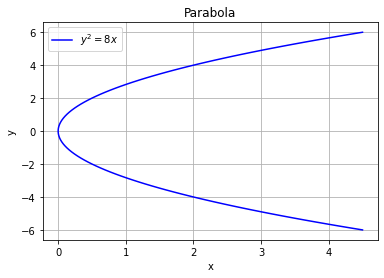
\includegraphics[width=\columnwidth]{Assignment-5.png}
    \caption{Plot of the parabola}
    \label{plot}
\end{figure}
\end{document}